% System Parameters
% Outline any system parameters and variables required by the system

% Flowcharts
% Include a flowchart diagram for each major function in your code, including your two algorithms
% Describe how each algorithm works
\section{Create a Solution}
\begin{itemize}
    \item system parameters: none
    \item Flowcharts:
        \begin{figure}[H]
            \centering
            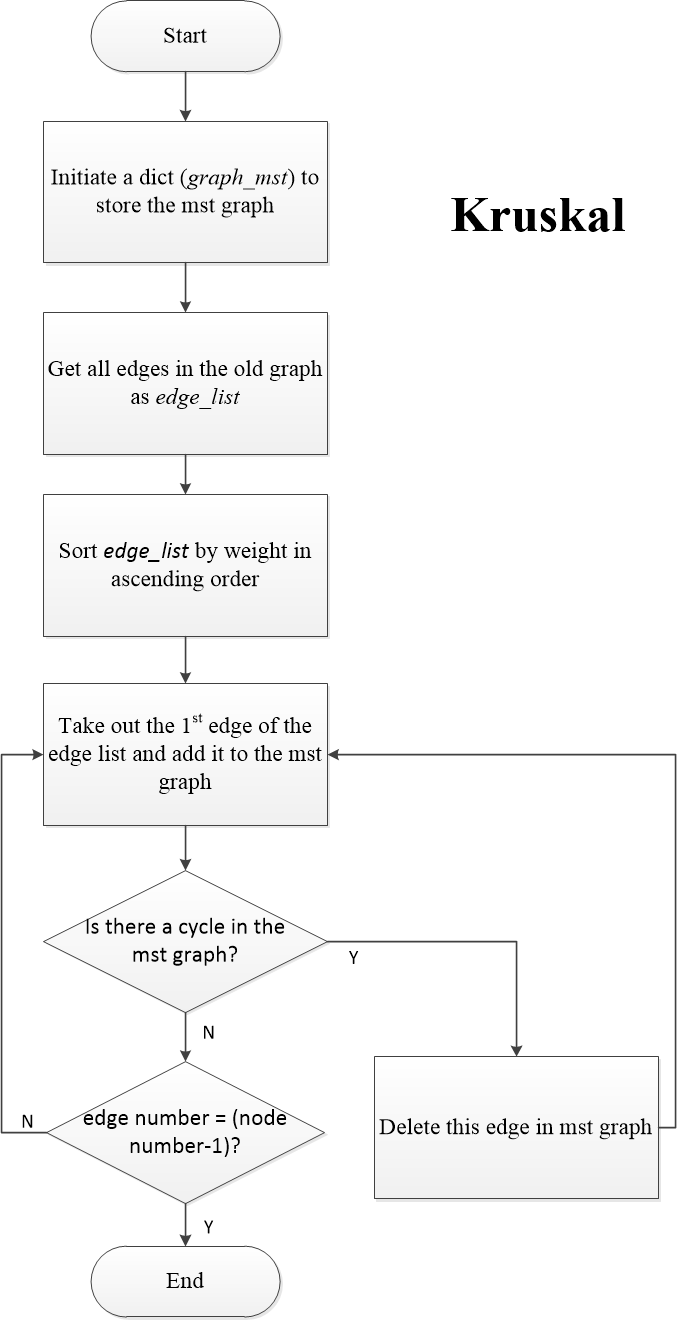
\includegraphics[width=0.8\linewidth, height=24cm]{figures\\flowchartKruskal.png}
            \caption{Flowchart-Kruskal}
            \label{fig:flowchart of Kruskal}
        \end{figure}

        \begin{figure}[H]
            \centering
            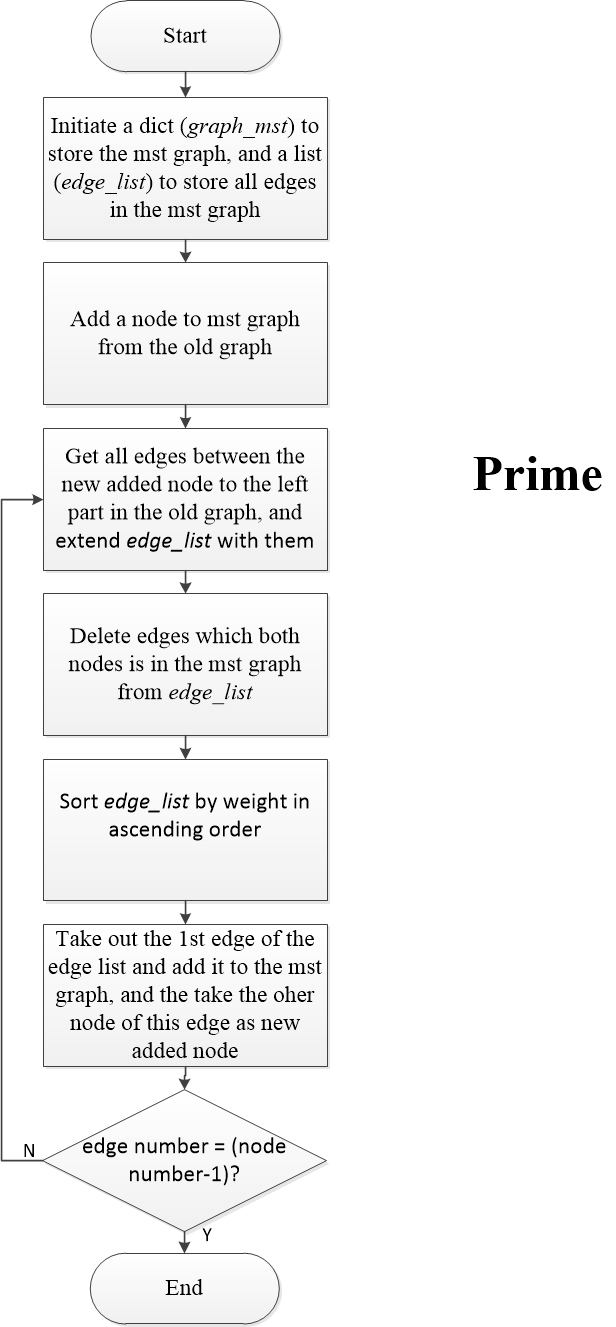
\includegraphics[width=0.8\linewidth, height=24cm]{figures\\flowchartPrime.png}
            \caption{Flowchart-Prime}
            \label{fig:flowchart of Prime}
        \end{figure}

        \begin{figure}[H]
            \centering
            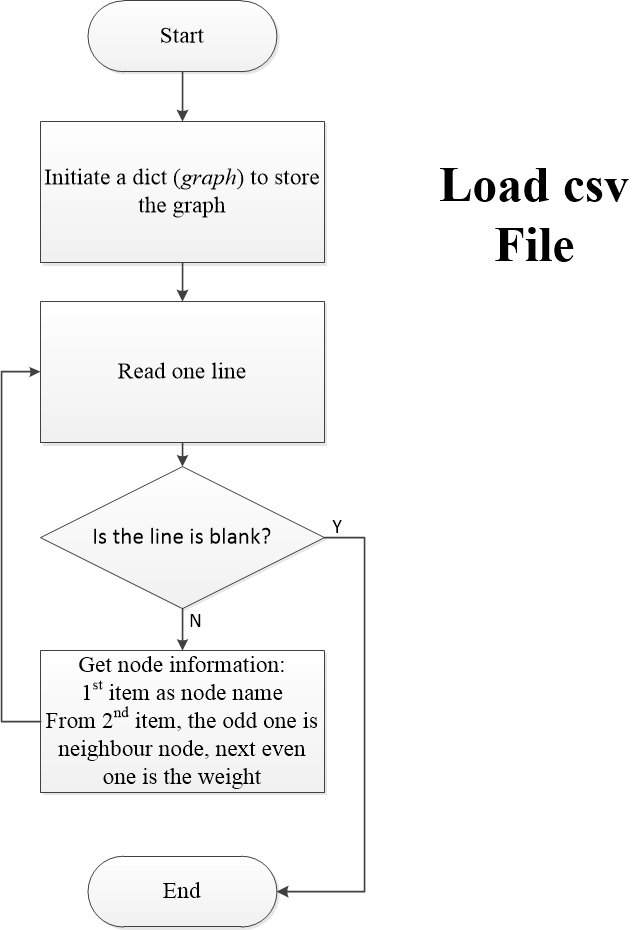
\includegraphics[width=0.8\linewidth, height=24cm]{figures\\flowchartLoadcsv.png}
            \caption{Flowchart-Load csv file}
            \label{fig:flowchart of Load csv}
        \end{figure}

        \begin{figure}[H]
            \centering
            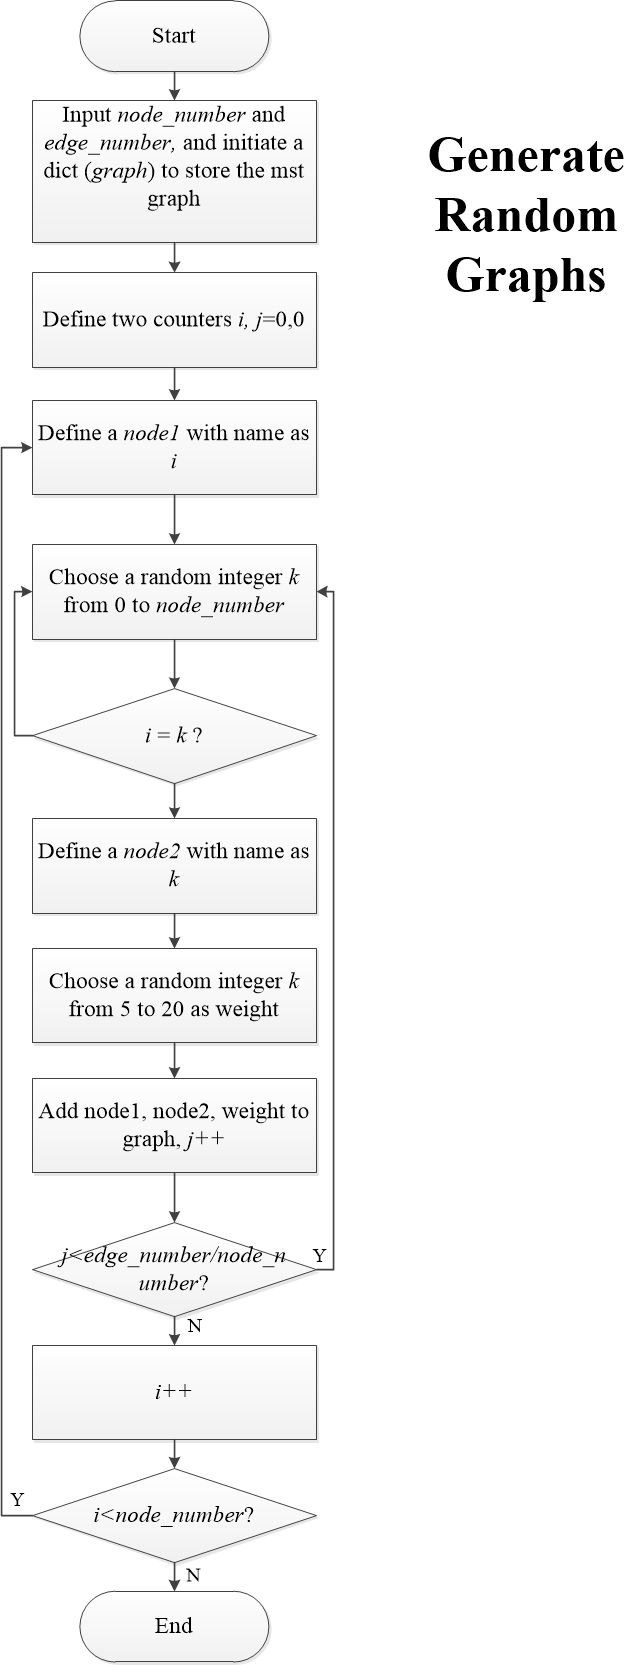
\includegraphics[width=0.8\linewidth, height=24cm]{figures\\flowchartGenerateRandomGraphs.png}
            \caption{Flowchart-Generate Random Graphs}
            \label{fig:flowchart of Generate Random Graphs}
        \end{figure}


    \item Descriptions:
        \begin{itemize}
            \item Kruskal:
                \begin{enumerate}
                    \item Get all edges from the old graph
                    \item Sort edge list by weight in ascending order
                    \item Take out the 1st edge of the edges and add it to the mst graph
                    \item Judge if there are cycles in mst graph, if so, delete it
                    \item judge if the number of edges is enough (node number -1 ), if so, we already get the result, else, back to step3
                \end{enumerate}
            \item Prime:
                \begin{enumerate}
                    \item Add a node to mst graph from the old graph
                    \item Get all edges between the new added node to the left part in the old graph, and extend edge list with them
                    \item Delete edges which both nodes is in the mst graph from edge list
                    \item Sort edge list by weight in ascending order
                    \item Take out the 1st edge of the edge list and add it to the mst graph, and the take the oher node of this edge as new added node
                    \item judge if the number of edges is enough (node number -1 ), if so, we already get the result, else, back to step2
                \end{enumerate}
        \end{itemize}
\end{itemize}